\begin{frame}
\begin{block}{\textbf{Question}}
How can we find the constraints on $\mathbf{P}_{n \times 1}$ in order for $\mathbf{G}_{n \times m} \mathbf{Q}_{m \times 1} = \mathbf{P}_{n \times 1}$ to have a solution?
\end{block}
\begin{block}{\textbf{Cokernel}}
These constraints are defined by the cokernel of $\mathbf{G} \colon \mathcal{D}_R\mathcal{E}(L) \rightarrow \mathcal{D}_R\mathcal{E}(\mathcal{G})$
\begin{center}
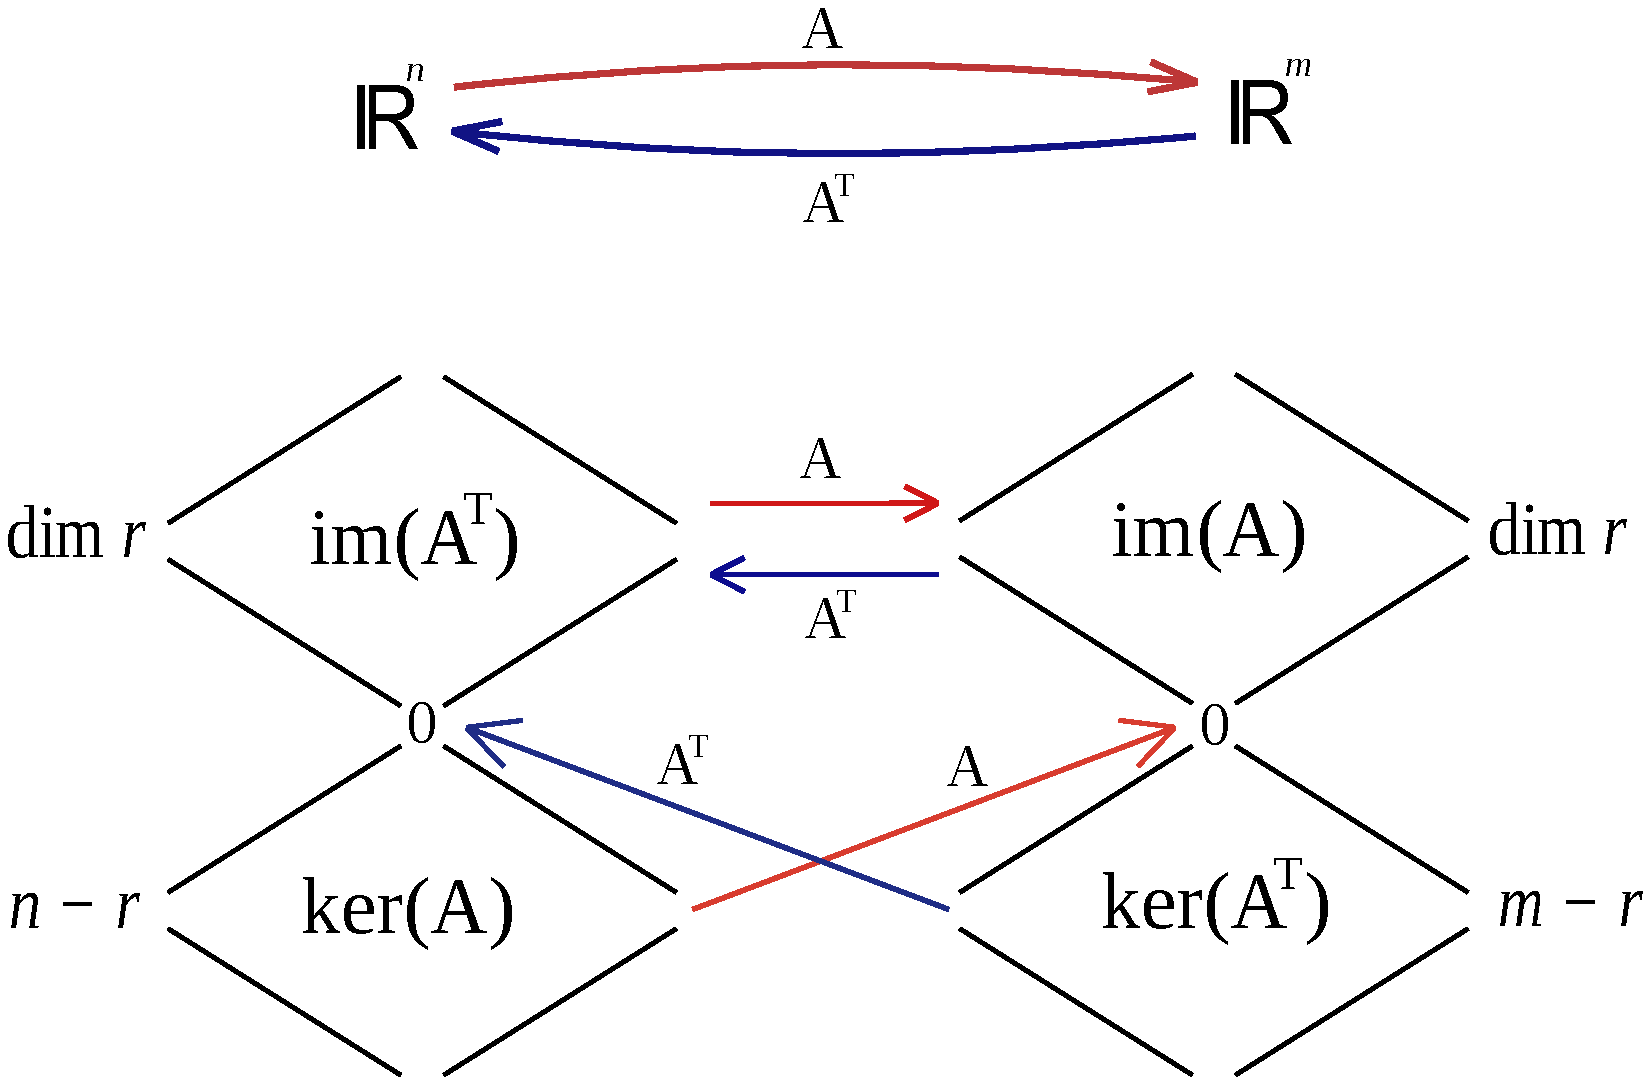
\includegraphics[width=0.5\textwidth]{fig/fundamental_subspaces.pdf}
\end{center}
\end{block}
\end{frame}

